\documentclass[11pt,letterpaper]{article}
\usepackage[T1]{fontenc}
\usepackage[utf8]{inputenc}
\usepackage{lmodern}
\usepackage[margin=0.75in,headheight=15pt,headsep=18pt,footskip=24pt]{geometry}
\usepackage{microtype,amsmath,amssymb,mathtools,booktabs,tabularx,array}
\usepackage{xcolor,tikz,tcolorbox,enumitem,fancyhdr,titlesec,listings,caption,hyperref}
\newcolumntype{Y}{>{\raggedright\arraybackslash}X}
\usetikzlibrary{arrows.meta,positioning,calc,fit,decorations.pathmorphing}
\definecolor{navy}{HTML}{17324D}
\definecolor{teal}{HTML}{087E8B}
\definecolor{pale}{HTML}{EDF6F7}
\definecolor{orange}{HTML}{D87828}
\definecolor{graytext}{HTML}{526171}
\definecolor{lightgray}{HTML}{F3F5F7}
\hypersetup{colorlinks=true,linkcolor=teal,urlcolor=teal,citecolor=teal,pdftitle={EC523 Project B: Remove the Noise, Keep the Voice},pdfauthor={EC523 course staff},pdfsubject={Deep-learning project in single-channel speech enhancement}}
\pagestyle{fancy}
\fancyhf{}
\fancyhead[L]{\small\sffamily\color{navy}EC523 / FALL 2026}
\fancyhead[R]{\small\sffamily\color{graytext}PROJECT B / COURSE PROJECT}
\fancyfoot[L]{\footnotesize\color{graytext}Single-channel speech enhancement}
\fancyfoot[R]{\footnotesize\thepage}
\renewcommand{\headrulewidth}{0.3pt}
\setlength{\parindent}{0pt}
\setlength{\parskip}{6pt}
\setlist[itemize]{leftmargin=1.3em,itemsep=3pt,topsep=3pt}
\setlist[enumerate]{leftmargin=1.6em,itemsep=4pt,topsep=3pt}
\titleformat{\section}{\Large\sffamily\bfseries\color{navy}}{\thesection}{0.6em}{}
\titleformat{\subsection}{\normalsize\sffamily\bfseries\color{teal}}{}{0pt}{}
\titlespacing*{\section}{0pt}{0pt}{10pt}
\titlespacing*{\subsection}{0pt}{9pt}{3pt}
\captionsetup{font=small,labelfont=bf,skip=5pt,hypcap=false}
\tcbset{colback=pale,colframe=teal,boxrule=0.5pt,arc=2pt,left=8pt,right=8pt,top=5pt,bottom=5pt,before skip=8pt,after skip=8pt}
\lstset{basicstyle=\ttfamily\small,backgroundcolor=\color{lightgray},frame=single,rulecolor=\color{lightgray},breaklines=true,columns=fullflexible,keepspaces=true,showstringspaces=false,xleftmargin=5pt,xrightmargin=5pt}
\newcommand{\page}[1]{\clearpage\section{#1}}
\newcommand{\R}{\mathbb{R}}
\newcommand{\clip}{\operatorname{clip}}
\newcommand{\smallnote}[1]{{\small\color{graytext}#1\par}}
\tikzset{box/.style={draw=teal,fill=pale,rounded corners=2pt,minimum height=0.65cm,align=center,font=\small},arr/.style={-{Latex[length=2mm]},thick,color=navy}}
\begin{document}
\setcounter{section}{1}

{\sffamily\color{teal}\large PROJECT B \hfill Teams of three}
\vspace{6pt}

{\sffamily\bfseries\color{navy}\fontsize{29}{33}\selectfont Remove the Noise,\par Keep the Voice\par}
\vspace{5pt}
{\Large\sffamily Learning to remove noise without damaging speech\par}

\begin{tcolorbox}
\textbf{The research question.} Given noisy speech $x$ and its paired clean target $y$, can a deep-learning idea remove background noise while preserving intelligibility, speaker characteristics, and naturalness? An enhancer succeeds only if the speech sounds better without new artifacts.
\end{tcolorbox}

\subsection{Denoising is a three-way tradeoff}
Returning the input preserves every word and every noise. Aggressive suppression removes noise but can erase consonants, flatten pitch, or create ``musical noise.'' A good enhancer must suppress interference, preserve speech, and avoid inventing structure. No single objective metric fully settles that tradeoff.

\begin{center}
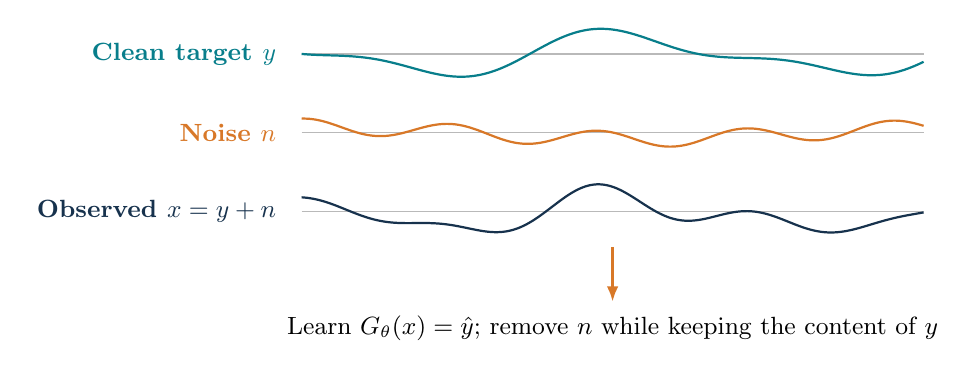
\begin{tikzpicture}[x=1cm,y=1cm]
\foreach \yy/\name/\col in {2.0/Clean target $y$/teal,1.0/Noise $n$/orange,0.0/Observed $x=y+n$/navy}{
  \draw[gray!55] (2.3,\yy)--(10.2,\yy);
  \node[anchor=east,font=\small\bfseries,text=\col] at (2.1,\yy) {\name};
}
\draw[teal,thick,samples=220,smooth,domain=2.3:10.2] plot (\x,{2+.24*sin(70*\x)+.11*sin(137*\x)});
\draw[orange,thick,samples=220,smooth,domain=2.3:10.2] plot (\x,{1+.10*sin(193*\x)+.08*sin(41*\x)});
\draw[navy,thick,samples=220,smooth,domain=2.3:10.2] plot (\x,{.24*sin(70*\x)+.11*sin(137*\x)+.10*sin(193*\x)+.08*sin(41*\x)});
\draw[orange,very thick,-{Latex[length=2mm]}] (6.25,-.45)--(6.25,-1.15);
\node[font=\small,align=center] at (6.25,-1.48) {Learn $G_\theta(x)=\hat y$; remove $n$ while keeping the content of $y$};
\end{tikzpicture}
\captionof{figure}{A conceptual additive mixture, not a dataset recording. After removing the vertical display offsets, the bottom trace is exactly the sample-by-sample sum of the top two traces. Real recordings can also contain reverberation and nonlinear distortion.}
\end{center}

\subsection{What you will build}
Start from a common time-frequency baseline and make \textbf{one hypothesis-driven modification}: for example, change the learning objective, model phase, or combine local and long-range spectral context. Submit one checkpoint, code, a report, and listening examples. The submitted enhancer is run through one fixed command on noisy and clean inputs.

\begin{tcolorbox}[colback=lightgray,colframe=graytext]
\textbf{What the course provides.} You receive a versioned paired dataset, fixed split manifests, a trained baseline, the scoring environment, and a small untrained model that demonstrates the submission interface. The interface demo is not a competitive enhancer.
\end{tcolorbox}
\smallnote{Reading route: signal concepts, Section~2; research directions, Section~3; project and data, Sections~4--5; evaluation, Sections~6--8; submission, Section~9; research and grading, Sections~10--11; readings and checklist, Section~12.}

\page{From waveform to time-frequency mask and back}
\subsection{The signals and their shapes}
After staff preprocessing, an utterance is a mono sequence $x\in[-1,1]^T$ sampled at $f_s=16{,}000$ samples/second. Its paired clean reference $y\in[-1,1]^T$ has the \emph{same length and alignment}. The common approximation is
\begin{equation}
x[t]=y[t]+n[t],\qquad t=0,\ldots,T-1,
\end{equation}
but recorded distortions may include reverberation and nonlinear effects that do not separate neatly into $y+n$.

The short-time Fourier transform (STFT) divides a waveform into overlapping windows. For frame $m$ and frequency bin $k$,
\begin{equation}
X[m,k]=\sum_{t=0}^{L-1}x[t+mh]w[t]e^{-j2\pi kt/L}=|X[m,k]|e^{j\angle X[m,k]}.
\end{equation}
$L$ is the window length, $h$ the hop, and $w$ the analysis window. The magnitude $|X|$ describes how much energy lies in each time-frequency cell; $\angle X$ is phase. With $L=512$ at 16 kHz, one window spans 32 ms and a one-sided spectrum has 257 bins.

\begin{center}
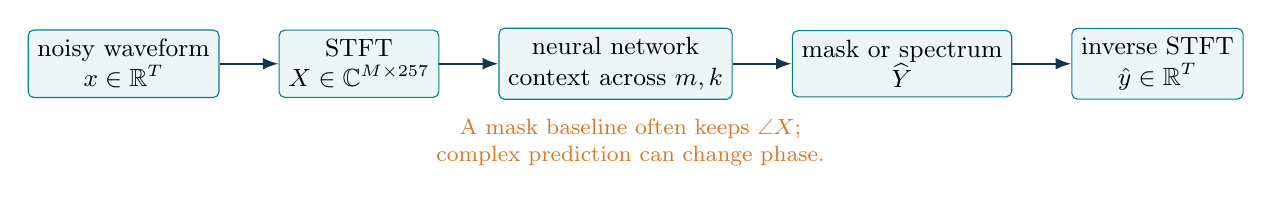
\begin{tikzpicture}[node distance=.75cm]
\node[box] (wav) {noisy waveform\\$x\in\R^T$};
\node[box,right=of wav] (stft) {STFT\\$X\in\mathbb C^{M\times257}$};
\node[box,right=of stft] (net) {neural network\\context across $m,k$};
\node[box,right=of net] (mask) {mask or spectrum\\$\widehat Y$};
\node[box,right=of mask] (istft) {inverse STFT\\$\hat y\in\R^T$};
\draw[arr] (wav)--(stft);\draw[arr] (stft)--(net);\draw[arr] (net)--(mask);\draw[arr] (mask)--(istft);
\node[font=\footnotesize,text=orange,align=center] at ($(stft)!0.5!(mask)+(0,-1.0)$) {A mask baseline often keeps $\angle X$;\\complex prediction can change phase.};
\end{tikzpicture}
\captionof{figure}{The course baseline. STFT and inverse STFT are fixed signal-processing layers; the trainable network predicts what to keep or reconstruct.}
\end{center}

\subsection{A real mask baseline}
A magnitude-mask model predicts $M_\theta(X)\in[0,1]^{M\times257}$ and reconstructs
\begin{equation}
\widehat Y=M_\theta(X)\odot |X|e^{j\angle X},\qquad \hat y=\operatorname{iSTFT}(\widehat Y).
\end{equation}
This cannot directly correct noisy phase, and a $[0,1]$ mask cannot amplify a weak time-frequency cell. Those constraints make the baseline understandable, not universally optimal. A complex mask, direct complex-spectrum prediction, or waveform model changes the output space and must be evaluated fairly.

\subsection{Why sample-wise loss is not enough}
Waveform $L_1$, magnitude $L_1$, and multi-resolution spectral losses are useful because they are stable and differentiable. Yet two signals can be close in squared error and sound different, while a harmless gain change can increase squared error. ``Perceptual'' is a claim about listeners; a convenient loss is only a proxy.

\page{Three research directions}
The project is about a speech-enhancement question, not the reproduction of one paper. Choose one of the directions below, combine them only when the combined hypothesis can be tested cleanly, or propose another idea of comparable depth.

\begin{center}
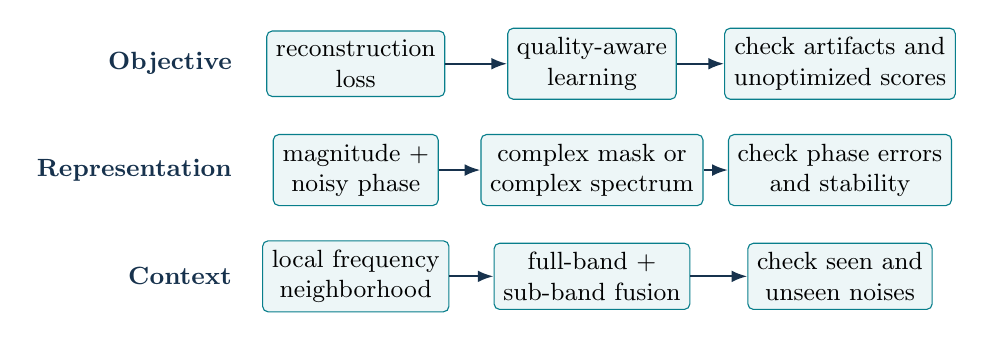
\begin{tikzpicture}[x=1cm,y=1cm]
\node[font=\small\bfseries,text=navy,anchor=east] at (1.65,1.35) {Objective};
\node[box] (rec) at (3.1,1.35) {reconstruction\\loss};
\node[box] (qual) at (6.1,1.35) {quality-aware\\learning};
\node[box] (qtest) at (9.25,1.35) {check artifacts and\\unoptimized scores};
\draw[arr] (rec)--(qual); \draw[arr] (qual)--(qtest);

\node[font=\small\bfseries,text=navy,anchor=east] at (1.65,0) {Representation};
\node[box] (mag) at (3.1,0) {magnitude +\\noisy phase};
\node[box] (complex) at (6.1,0) {complex mask or\\complex spectrum};
\node[box] (ptest) at (9.25,0) {check phase errors\\and stability};
\draw[arr] (mag)--(complex); \draw[arr] (complex)--(ptest);

\node[font=\small\bfseries,text=navy,anchor=east] at (1.65,-1.35) {Context};
\node[box] (local) at (3.1,-1.35) {local frequency\\neighborhood};
\node[box] (fusion) at (6.1,-1.35) {full-band +\\sub-band fusion};
\node[box] (ctest) at (9.25,-1.35) {check seen and\\unseen noises};
\draw[arr] (local)--(fusion); \draw[arr] (fusion)--(ctest);
\end{tikzpicture}
\captionof{figure}{Three defensible starting points. Each row pairs a model change with evidence needed to support the claim. The arrows show a forward design path; they are not gradient paths.}
\end{center}

\subsection{Direction A: change what the model learns to value}
Sample and spectral reconstruction losses reward numerical similarity, but they do not fully describe perceived speech quality. One option is to learn a differentiable quality predictor $q_\phi(y,s)$ that approximates a fixed, non-differentiable score $m(y,s)$ for clean reference $y$ and candidate $s$. The enhancer $G_\theta$ can then use
\begin{equation}
L_G=\lambda_{\rm rec}L_{\rm rec}(G_\theta(x),y)
+\lambda_{q}\bigl[q_\phi(y,G_\theta(x))-1\bigr]^2.
\end{equation}
This is the broad idea behind MetricGAN+~\cite{metricgan}. It is not the only possible objective: a carefully tested multi-resolution spectral loss, phase-sensitive loss, or clean-preservation loss can also support a strong project.

The danger is reward hacking. If $q_\phi$ is wrong outside its training examples, the enhancer may discover artifacts that fool it. A quality-aware project must compare against reconstruction-only training, measure predictor error on untouched examples, report an unoptimized metric, and show failures where predicted and measured quality disagree.

\subsection{Direction B: represent phase instead of inheriting it}
The baseline estimates magnitude and copies the noisy phase. DCCRN instead processes complex spectra and estimates a complex ratio mask~\cite{dccrn}. This gives the model a way to correct phase, which can matter when speech and noise overlap strongly. It also creates a harder optimization problem: unstable phase estimates can introduce audible distortion. A clean test holds the data, loss, training budget, and backbone scale as close as possible while changing the output representation.

\subsection{Direction C: combine global and local spectral context}
Speech has structure at two useful scales. Nearby frequency bins reveal local harmonics and noise patterns, while the full spectrum gives context about the frame as a whole. FullSubNet combines a full-band model with sub-band processing to use both~\cite{fullsubnet}. A student version need not reproduce the full system. It might compare a sub-band module with and without a compact full-band summary under the same parameter budget. Break results down by noise family: context that helps steady noise may fail on short, unfamiliar events.

\page{Project contract and design choices}
\small
\subsection{The common starting point}
The course baseline uses 16 kHz mono audio, a 512-sample STFT window, a 128-sample hop, a small two-layer BLSTM, a real $[0,1]$ magnitude mask, noisy phase, and a stated reconstruction loss. Reproduce its development result before changing it. The noisy input, common baseline, and your method must appear as separate rows in every main result table.

\begin{center}\small
\renewcommand{\arraystretch}{1.12}
\begin{tabularx}{\linewidth}{@{}>{\raggedright\arraybackslash}p{1.22in}YY@{}}
\toprule
Direction & Concrete starting experiment & What must be isolated\\\midrule
Quality-aware objective & Reconstruction vs. reconstruction + learned score surrogate & Surrogate coverage, replay, held-out measured scores\\
Mask/phase & Real mask vs. complex ratio mask & Same backbone, budget, and losses when possible\\
Temporal context & Add GRU, TCN, attention, or state-space bottleneck & Context block removed or compute-matched control\\
Clean preservation & Predict noise severity and blend $x$ with $G(x)$ & Gate/blend ablation; clean-input behavior\\
Robustness & SNR curriculum or noise augmentation & Matched training examples and unseen-noise breakdown\\
Efficiency & Distillation, pruning, causal or compact model & Quality, parameters, latency, RTF, memory\\
\bottomrule
\end{tabularx}
\end{center}

\subsection{What counts as the contribution?}
A U-Net, BLSTM, or another standard architecture may serve as a baseline or component. Using one is not, by itself, a research contribution. Your proposal must identify a mechanism, predict a measurable result, and isolate one major change. For example: ``complex phase correction should improve waveform fidelity at low SNR, but unstable phase estimates may reduce perceived quality.''

\subsection{Main-track rules}
\begin{itemize}
\item One submitted checkpoint and one deterministic inference path for every utterance. No target audio, transcript, filename-specific behavior, network access, test-time training, or ensemble selected by evaluation condition.
\item Train only on the released training partition and explicitly allowed resources. Do not use the official public test targets for training, tuning, or model selection. External pretrained enhancement, speech, or quality models are disallowed in the main track unless staff list them.
\item Output mono 16 kHz audio with exactly the input length. Do not clip, independently renormalize each output, or shift it to improve a metric. The model may learn gain, but the evaluation waveform is exactly what the CLI writes.
\item Main-track limit: at most 15M trainable parameters and 32 GiB peak allocated training memory on one L40S. The course site gives the per-team GPU-hour allocation and server timeout.
\end{itemize}

\subsection{A feasible first route}
Verify paired alignment and overfit a few crops. Reproduce the baseline, implement one modification, run a small development sweep, and freeze the comparison. Four-second aligned crops, mixed precision, accumulation, and cached metric labels are reasonable tools; the black-box metric need not run in every mini-batch.

\normalsize
\page{Data and a protocol that resists leakage}
\subsection{The paired speech collection}
The University of Edinburgh database provides parallel clean/noisy speech derived from VCTK and several noise sources, including DEMAND~\cite{dataset}. The course-scale source is the 28-speaker training set; the commonly used test set contains speech from two unseen speakers. The source archive is 48 kHz. Staff will distribute a versioned 16 kHz course package with checksums and manifests. The larger 56-speaker version is not part of the main track.

The standard VoiceBank-DEMAND setup has 11,572 paired training utterances and 824 paired test utterances; common training mixtures use 0, 5, 10, and 15 dB SNR, while the standard test uses intermediate SNRs~\cite{metricgan}. Exact course counts may differ after integrity checks and staff-held partitions; the manifest, not an assumed filename convention, is authoritative.

\subsection{Course partitions}
\begin{center}\small
\begin{tabularx}{\linewidth}{@{}p{1.1in}p{1.45in}Y@{}}
\toprule
Partition & Available to teams? & Purpose\\\midrule
Train & noisy + clean & Fit model weights and any quality surrogate.\\
Development & noisy + clean & Choose settings; publish baseline and metric examples. Group by speaker.\\
Public evaluation & inputs; labels scored by server & Limited feedback on the exact scoring code.\\
Private evaluation & no files or labels & Final ranking using held-out utterance/noise combinations.\\
Clean preservation & private clean inputs & Detect enhancement artifacts when no removal is needed.\\
\bottomrule
\end{tabularx}
\end{center}

Renaming public files does not make them secret. The private mixtures therefore use unreleased noise excerpts, SNRs, and mixing seeds, and the split is checked for speaker and content overlap. A submission-quality paper should also include an independent corpus or authorized held-out evaluation instead of treating a course split as proof of broad generalization.

\subsection{Fixed preprocessing}
Staff perform conversion once: decode the source PCM, downmix only when required, resample with one published polyphase implementation, and store float-equivalent 16-bit PCM WAV at 16 kHz. Paired files receive the same trimming and timing decisions. Reject a pair whose alignment or length cannot be verified. Do not independently peak-normalize clean and noisy files; that changes their physical relationship.

During training, crop or pad the clean/noisy pair with the same indices. Evaluation uses the full utterance. Silence is part of the signal and must not be deleted. No voice-activity trimming, loudness normalization, or delay correction occurs after a team produces its output.

\subsection{What may be reported beyond the course benchmark?}
Teams may report the standard public test set as a clearly labeled secondary comparison, provided it never influences the course-private model choice. CSIG, CBAK, and COVL may be included for historical comparison with MetricGAN+, but they are regression estimators, not new listener ratings and not independent leaderboard components. Any listening study that collects human-subject data requires instructor and institutional guidance; informal classroom examples are qualitative evidence only.

\page{Evaluation I: perceptual quality and intelligibility}
For each utterance $i$, let $y_i$ be the clean reference and $\hat y_i$ the submitted output. Metrics are computed at 16 kHz on the exact aligned arrays written by the runner. Each utterance receives equal weight, regardless of duration.

\subsection{1. Wideband PESQ: a perceptual-quality predictor}
PESQ (Perceptual Evaluation of Speech Quality) compares a level-aligned, perceptually transformed reference and degraded signal and predicts a MOS-like quality score~\cite{pesq}. The course pins the public Python package \texttt{pesq} version 0.0.4 and uses ITU-T P.862.2 wideband mode at 16 kHz~\cite{pesqcode}:
\begin{equation}
p_i=\operatorname{PESQ}_{\rm WB}(y_i,\hat y_i),\qquad
P(D)=\frac1{|D|}\sum_{i\in D}\clip\!\left(\frac{p_i-1}{3.5},0,1\right).
\end{equation}
The affine transform maps 1 to 0 and 4.5 to 1; clipping makes the leaderboard component bounded. It does \emph{not} turn PESQ into a probability or true human MOS. PESQ performs internal perceptual processing and alignment, but teams may not shift outputs before scoring.

The P.862 family was withdrawn in 2024 in favor of ITU-T P.863~\cite{itupesq}. We retain wideband P.862.2 because it remains the comparison used by much of the VoiceBank-DEMAND literature. Treat it as a benchmark measure, not a current telecommunications recommendation or a substitute for listening.

\subsection{2. STOI: predicted intelligibility}
STOI compares short-time temporal envelopes in one-third-octave bands and was designed for noisy and time-frequency-weighted speech~\cite{stoi}. Conceptually, let $a_{j,m}\in\R^N$ be a clean envelope segment and $b_{j,m}$ the corresponding enhanced segment after STOI's normalization and clipping. Their correlation is
\begin{equation}
d_{j,m}=\frac{(a_{j,m}-\bar a_{j,m}\mathbf1)^\top(b_{j,m}-\bar b_{j,m}\mathbf1)}
{\|a_{j,m}-\bar a_{j,m}\mathbf1\|_2\,\|b_{j,m}-\bar b_{j,m}\mathbf1\|_2}.
\end{equation}
The implementation averages valid $d_{j,m}$ values over bands $j$ and segments $m$ to obtain $s_i=\operatorname{STOI}(y_i,\hat y_i)$. Ranking uses
\begin{equation}
S(D)=\frac1{|D|}\sum_{i\in D}\clip(s_i,0,1).
\end{equation}
The displayed equation explains the correlation core; the pinned evaluator defines resampling, silent-frame removal, octave bands, normalization, clipping, and numerical tolerances. A STOI value is an index correlated with intelligibility, not ``the percentage of words understood.''

\begin{center}
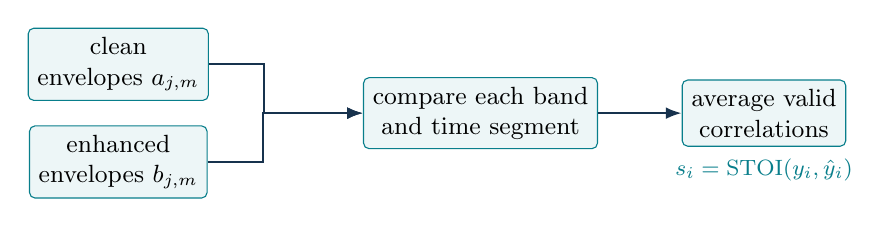
\begin{tikzpicture}[x=1cm,y=1cm]
\node[box] (ref) at (1.5,.62) {clean\\envelopes $a_{j,m}$};
\node[box] (est) at (1.5,-.62) {enhanced\\envelopes $b_{j,m}$};
\node[box] (corr) at (6.1,0) {compare each band\\and time segment};
\node[box] (avg) at (9.7,0) {average valid\\correlations};
\draw[arr] (ref.east)--++(.7,0)|-(corr.west);
\draw[arr] (est.east)--++(.7,0)|-(corr.west);
\draw[arr] (corr)--(avg);
\node[font=\footnotesize,text=teal] at (9.7,-.72) {$s_i=\operatorname{STOI}(y_i,\hat y_i)$};
\end{tikzpicture}
\captionof{figure}{Both envelope streams enter the comparison. STOI averages their short-time correlations; it does not infer words or replace listening.}
\end{center}

\page{Evaluation II: signal fidelity and the exact score}
\subsection{3. Scale-invariant signal-to-distortion ratio}
First subtract each signal's sample mean. For a nonzero reference $y_i$, project $\hat y_i$ onto it:
\begin{align}
\alpha_i&=\frac{\hat y_i^\top y_i}{\|y_i\|_2^2},&
e_{\rm target}&=\alpha_i y_i,&
e_{\rm residual}&=\hat y_i-e_{\rm target},\\
r_i&=10\log_{10}\frac{\|e_{\rm target}\|_2^2+\epsilon}{\|e_{\rm residual}\|_2^2+\epsilon}.
\end{align}
This is SI-SDR~\cite{sisdr}. It ignores one global gain, so it must be paired with output bounds and clean preservation. We cap extreme values only for aggregation:
\begin{equation}
R(D)=\frac1{|D|}\sum_{i\in D}\frac{\clip(r_i,-10,30)+10}{40}.
\end{equation}
Thus $-10$ dB maps to 0, 30 dB maps to 1, and intermediate values are linear. Raw uncapped SI-SDR is always reported. The evaluator fixes $\epsilon=10^{-8}$ after signals are represented as float64 in $[-1,1]$.

\subsection{Quality on any specified collection}
All three normalized components lie in $[0,1]$:
\begin{equation}
\boxed{A(D)=0.40P(D)+0.30S(D)+0.30R(D).}
\end{equation}
The perceptual-quality term receives the largest individual weight, while intelligibility and signal fidelity together carry more weight. This makes it harder to win by exploiting one score. The weights, caps, modes, and averaging rules are fixed before the competition.

\subsection{Clean-input preservation}
For each private clean utterance $y_i$, staff also run the enhancer with input $x_i=y_i$. Let $c_i=G_\theta(y_i)$ and evaluate it against $y_i$ using exactly the same $A$. Denote that collection $D_{\rm clean}$. An identity mapping should be nearly perfect; an enhancer that colors or suppresses already-clean speech loses credit.

The private noisy collection $D_{\rm noisy}$ contains held-out utterance/noise/SNR combinations. The leaderboard score is
\begin{equation}
\boxed{\operatorname{Score}=100\left[0.85A(D_{\rm noisy})+0.15A(D_{\rm clean})\right].}
\end{equation}
The range is 0--100. There is no hidden multiplier and no reward for deliberately weakening the baseline. The public leaderboard uses the same formula on its public/private-feedback partition; final ranking uses the nominated checkpoint on the private instances.

\begin{center}
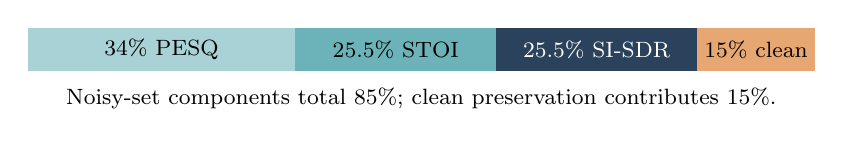
\begin{tikzpicture}[x=1cm,y=1cm]
\fill[teal!35] (0,0) rectangle (3.4,.55);\node[font=\footnotesize] at (1.7,.275) {34\% PESQ};
\fill[teal!60] (3.4,0) rectangle (5.95,.55);\node[font=\footnotesize] at (4.675,.275) {25.5\% STOI};
\fill[navy!92] (5.95,0) rectangle (8.5,.55);\node[font=\footnotesize,text=white] at (7.225,.275) {25.5\% SI-SDR};
\fill[orange!65] (8.5,0) rectangle (10,.55);\node[font=\footnotesize] at (9.25,.275) {15\% clean};
\node[font=\footnotesize] at (5,-.35) {Noisy-set components total 85\%; clean preservation contributes 15\%.};
\end{tikzpicture}
\captionof{figure}{Final score allocation after expanding the nested weights. The clean component itself contains the same 40/30/30 quality mixture.}
\end{center}

\page{Evaluation III: validity, diagnostics, and leaderboard policy}
\subsection{Waveform validity is checked before metrics}
For every manifest ID, output must be a mono 16 kHz WAV with exactly the input sample count, finite samples, and peak absolute value at most 1.0 after decoding. Missing, extra, stereo, clipped, NaN, delayed, shortened, or resampled outputs invalidate the run. Staff do not repair an output. File IDs, source/output hashes, model hash, environment, latency, and peak statistics enter a run manifest.

Silence-only references are excluded by the released evaluation manifest. If a metric still fails on a valid file, the entire run is held for staff diagnosis rather than silently dropping the utterance. Scores are means of per-utterance metrics; do not concatenate audio or duration-weight the mean.

\subsection{Public feedback and final ranking}
Thirty percent of the course-evaluation instances provide public feedback; the remaining 70\% are used only for the final private run. Both portions are balanced across speakers, noise families, and SNR ranges. The server accepts at most two submissions per team per day and one nominated checkpoint for the final run. Final results are ranked at full precision, with mean ranks for exact ties. Private clean targets and per-example metric logs are never released.

Every team must make one server submission at the midpoint. This is an engineering checkpoint: it confirms that the model, checkpoint, and command work together on the evaluation server. The midpoint table reports scores to each team but \textbf{does not rank teams and does not contribute ranking points}. The ranked competition begins after the midpoint review.

Because the source corpus is public, these controls reduce leakage but cannot make it impossible. The private set uses newly mixed noise excerpts, and source and checkpoint provenance are audited. A team that uses evaluation targets, memorizes evaluation identities, or queries an external enhancement service is ineligible.

\subsection{Required diagnostics, not extra score terms}
\begin{itemize}
\item Raw noisy input, common baseline, and proposal: PESQ, STOI, raw SI-SDR, and the composite, with per-SNR and per-noise-family breakdowns.
\item Paired bootstrap 95\% intervals over utterance IDs for proposal-minus-baseline differences. Do not bootstrap individual samples or STFT frames.
\item Parameter count, multiply-accumulate estimate or FLOPs convention, L40S peak allocated inference/training memory, latency, and real-time factor (RTF = processing seconds / audio seconds). Warm-up and timing protocol must be stated.
\item Peak amplitude, clipped-sample count, DC offset, and clean-input results. Include unselected waveforms, spectrograms, and listening examples for improvements and failures.
\item For metric-aware methods: predicted-versus-true scatter, held-out calibration error and rank correlation, a replay or surrogate ablation, and failures where metrics disagree.
\end{itemize}

\subsection{What the score cannot establish}
PESQ, STOI, and SI-SDR are intrusive objective proxies. They do not directly identify speaker identity, phoneme errors, musical noise, listener preference, fairness across accents, or real-world microphone robustness. A high score does not prove naturalness, intelligibility for all listeners, or publication novelty. Make claims no broader than the evidence.

\page{Submission interface: one command, one checkpoint}
\subsection{The evaluation runner owns loading, file iteration, and validation}
Your team implements \texttt{submission/model.py} and supplies safe tensor weights. The evaluator invokes:
\begin{lstlisting}
python enhance.py --checkpoint submission/model.safetensors \
  --input evaluation/noisy --output predictions --device cuda
\end{lstlisting}
The input directory contains WAV files under nested IDs; the output mirrors those relative paths. The runner passes one waveform at a time as a float32 tensor of shape $1\times T$ at 16 kHz. Your model returns one tensor with the same shape. It receives no clean reference, filename, SNR, speaker ID, transcript, evaluation condition, or target score.

\begin{center}\small
\begin{tabularx}{\linewidth}{@{}p{2.05in}Y@{}}
\toprule
Student interface & Responsibility\\\midrule
\texttt{build\_enhancer}\newline\texttt{(sample\_rate)} & Construct all trainable modules once. Must support 16 kHz and expose no downloads or global model cache.\\
\texttt{enhance}\newline\texttt{(waveform, sample\_rate)} & Transform a $1\times T$ waveform without changing length. Deterministic in evaluation mode. No target or metadata.\\
\texttt{model.safetensors} & One checkpoint matching the source. No pickled code, alternate condition-specific checkpoints, or hidden assets.\\
\bottomrule
\end{tabularx}
\end{center}

\subsection{Files the runner produces}
For input \texttt{speaker/utt.wav}, the output is \texttt{speaker/utt.wav}. A \texttt{run.json} records input/output SHA-256, source and checkpoint hashes, sample counts, peak values, parameter count, device, elapsed time, audio duration, and RTF. The runner rejects duplicate IDs and unsafe paths.

\subsection{Use the interface demo before training}
\begin{lstlisting}
python make_demo.py --output demo
python enhance.py --checkpoint demo/model.safetensors \
  --input demo/noisy --output demo/enhanced --device cpu
python -m unittest discover -s tests -v
\end{lstlisting}
The demo synthesizes a few speech-like tones and noise, writes random/untrained weights, and checks the file contract. It is not real speech, does not train, and must never be quoted as performance. Official scoring additionally requires the staff-pinned PESQ/STOI environment.

\subsection{What the evaluator checks}
The run is reproduced in an isolated offline environment. The checks include source and parameter provenance, output hashes across repeated runs, and clean, quiet, long, short, and amplitude-edge inputs. A valid command-line interface does not prove scientific originality; the report, controlled comparisons, and individual explanation remain essential.

\page{Experiments: turn an implementation into evidence}
\subsection{Minimum controlled study}
\begin{enumerate}
\item \textbf{Sanity ladder.} Evaluate clean reference, noisy input, and common baseline. Confirm alignment, metric direction, length, gain, and several listened examples before interpreting a new model.
\item \textbf{One main comparison.} Train the baseline and proposed method with the same training partition and a declared model-selection rule. Match parameters or compute where feasible; report any mismatch rather than hiding it.
\item \textbf{One mechanism ablation.} Remove or replace the claimed idea: no quality surrogate, no complex phase, no context block, no clean gate, or no curriculum. A smaller performance drop than predicted is still an informative result.
\item \textbf{Generalization.} Break down unseen speaker, noise family, and SNR. Test the exact submitted checkpoint on clean inputs. Do not tune on the private leaderboard.
\item \textbf{Metric disagreement and failures.} Find cases where one metric improves while another worsens. Listen and inspect spectrograms for missing consonants, residual bursts, musical noise, reverberant tails, gain pumping, and speaker-coloration changes.
\item \textbf{Uncertainty and efficiency.} Report paired intervals, multiple seeds where affordable, parameters, memory, latency, and RTF. Distinguish variation across utterances from variation across training runs.
\end{enumerate}

\subsection{Individual understanding}
Each member must be able to explain the path from waveform to output, define the training losses and leaderboard metrics, trace tensor shapes, and predict what an ablation should change. For a quality-aware model, this includes the measured score $m$, learned predictor $q_\phi$, enhancer $G_\theta$, and which parameters are frozen during each alternating update.

\begin{tcolorbox}
\textbf{A strong claim is narrow and falsifiable.} Example: ``Replay training improves the chosen perceptual score at 0--5 dB SNR without reducing intelligibility, but the advantage disappears on transient unseen noise.'' The conclusion must show the relevant control, uncertainty, failures, and plausible alternative explanations.
\end{tcolorbox}

\subsection{Path from course project to paper}
The strongest work will explain a mechanism rather than stop at one leaderboard number. Useful next steps include compute-matched controls, repeated seeds, an independent corpus, and an appropriately approved listening study. A careful negative result can earn an excellent grade; publication is an ambition, not a grading requirement.

\subsection{Common traps}
Common failure modes include tuning to one score, comparing unequal data budgets, showing only hand-picked audio, dropping failed files from an average, calling STOI transcription accuracy, or describing a public test set as private. Noisy phase is not always wrong, complex prediction does not always help, and a learned score is not perceptual truth.

\page{Expectations, milestones, and grading}
\subsection{Teams and milestones}
Project B teams have \textbf{three students}. Rotate implementation, experiment, and interpretation roles so every member can explain the full system. Keep a contribution log with an owner and reviewer for every major experiment.

\begin{center}\small
\begin{tabularx}{\linewidth}{@{}p{1.55in}Y@{}}
\toprule
When & Expected work\\\midrule
September 28 & Project Pitch Day: a falsifiable question, chosen direction, main control, and smallest feasibility test.\\
Before November 2 & Complete the data/alignment tests, reproduce the baseline, run the CLI end to end, collect initial results, and measure L40S memory.\\
November 2 & Required midpoint submission: one server entry from every team plus a midway report with the method diagram, baseline and initial results, metric checks, resource use, risks, planned ablations, and each member's contribution. Midpoint results are not ranked.\\
December 14--18 & Final presentation, report, code, one checkpoint, and selected listening examples; exact slot to be confirmed. No assessment is due in the December 11--13 study period.\\
\bottomrule
\end{tabularx}
\end{center}
\smallnote{An early speech/STFT tutorial and baseline walkthrough provide the signal-processing background needed to begin before the later sequence-model lectures.}

\subsection{Project rubric (100 points)}
\begin{center}\small
\begin{tabularx}{\linewidth}{@{}p{.55in}p{1.75in}Y@{}}
\toprule
Points & Component & What earns credit\\\midrule
10 & Question and proposal & Specific hypothesis, relevant reading, clean comparison, feasible resource plan.\\
15 & Midway work & Valid paired pipeline, reproduced baseline, working modification, honest failures.\\
30 & Final research report & Correct method, fair controls, ablations, uncertainty, errors, limitations, supported claims.\\
15 & Reproducible implementation & Runnable code/weights, valid CLI, environment, hashes, logs, compute accounting.\\
15 & Presentation and individual understanding & Clear audio/visual evidence and questions; every member understands the system and metrics.\\
15 & Leaderboard component & Valid final entry plus competitive ranking, defined below.\\
\bottomrule
\end{tabularx}
\end{center}

For a valid final entry, assign $10+5(N-r)/(N-1)$ leaderboard points, where $N>1$ is the number of eligible teams and $r$ is rank (1 is best). Use mean ranks for exact ties. If $N=1$, assign 15. An invalid or missing entry receives 0 for this component, not automatically 0 for the project. The research work therefore remains most of the grade.

\subsection{Academic integrity and use of AI}
Follow the syllabus: AI may assist coding and research, but students own the creative decisions and must understand every submitted line. Write the report yourselves; AI use is limited to grammatical clarity. AI is not permitted for in-class presentations or quizzes. Cite external code, datasets, figures, pretrained components, and ideas; disclose tools and assistance. Never submit private audio to an external service or use evaluation targets for training or selection.

\page{Reading guide and final checklist}
\subsection{Three papers to understand before choosing a direction}
\begin{enumerate}
\item \textbf{MetricGAN+}~\cite{metricgan}: focus on the learned metric surrogate, noisy/clean examples, replay, and learnable sigmoid. Ask how surrogate error could mislead the enhancer.
\item \textbf{DCCRN}~\cite{dccrn}: a phase-aware complex convolutional recurrent model. Compare what a complex mask can express with the real-mask course baseline.
\item \textbf{FullSubNet}~\cite{fullsubnet}: combines full-band context with sub-band processing. Ask what each path contributes, and whether a smaller fusion module can isolate the same principle.
\end{enumerate}

\subsection{Before the final submission}
\begin{itemize}
\item One nominated checkpoint, source, pinned environment, training instructions, split manifest, and result table linked to seeds and hashes.
\item Noisy/baseline/proposal comparison; one mechanism ablation; clean-input test; raw and composite metrics; uncertainty; per-condition breakdowns.
\item Parameters, compute convention, training GPU-hours, L40S memory, latency/RTF; representative unselected waveforms, spectrograms, and failures.
\item Original report and slides in course templates with citations, limitations, contribution statement, and AI/code-use disclosure.
\item A fresh offline run of the exact command: no downloads, same output length, one checkpoint, no target or metadata access.
\end{itemize}

\footnotesize
\begin{thebibliography}{9}
\bibitem{metricgan} S.-W. Fu, C. Yu, T.-A. Hsieh, P. Plantinga, M. Ravanelli, X. Lu, and Y. Tsao. \emph{MetricGAN+: An Improved Version of MetricGAN for Speech Enhancement}. Interspeech, 2021. \url{https://arxiv.org/abs/2104.03538}.
\bibitem{dccrn} Y. Hu et al. \emph{DCCRN: Deep Complex Convolution Recurrent Network for Phase-Aware Speech Enhancement}. Interspeech, 2020. \url{https://arxiv.org/abs/2008.00264}.
\bibitem{fullsubnet} X. Hao, X. Su, R. Horaud, and X. Li. \emph{FullSubNet: A Full-Band and Sub-Band Fusion Model for Real-Time Single-Channel Speech Enhancement}. ICASSP, 2021. \url{https://arxiv.org/abs/2010.15508}.
\bibitem{dataset} C. Valentini-Botinhao. \emph{Noisy Speech Database for Training Speech Enhancement Algorithms and TTS Models}. University of Edinburgh DataShare, 2017. \url{https://doi.org/10.7488/ds/2117}.
\bibitem{voicebank} C. Valentini-Botinhao, X. Wang, S. Takaki, and J. Yamagishi. \emph{Speech Enhancement for a Noise-Robust Text-to-Speech Synthesis System Using Deep Recurrent Neural Networks}. Interspeech, 2016.
\bibitem{pesq} A. Rix, J. Beerends, M. Hollier, and A. Hekstra. \emph{Perceptual Evaluation of Speech Quality (PESQ)}. ICASSP, 2001; ITU-T P.862.2 wideband extension.
\bibitem{pesqcode} L. Malfait. \emph{pesq 0.0.4: Python wrapper for the PESQ score}. Public package and source code. \url{https://pypi.org/project/pesq/0.0.4/}.
\bibitem{itupesq} International Telecommunication Union. \emph{ITU-T Recommendation P.862}. Status and reference-code attachments. \url{https://www.itu.int/rec/T-REC-P.862}.
\bibitem{stoi} C. Taal, R. Hendriks, R. Heusdens, and J. Jensen. \emph{An Algorithm for Intelligibility Prediction of Time-Frequency Weighted Noisy Speech}. IEEE TASLP, 2011. \url{https://doi.org/10.1109/TASL.2011.2114881}.
\bibitem{sisdr} J. Le Roux, S. Wisdom, H. Erdogan, and J. Hershey. \emph{SDR -- Half-Baked or Well Done?} ICASSP, 2019. \url{https://arxiv.org/abs/1811.02508}.
\bibitem{l40s} NVIDIA. \emph{L40S GPU specifications}. \url{https://www.nvidia.com/en-us/data-center/l40s/}. Accessed August 31, 2026.
\end{thebibliography}
\end{document}
